\documentclass[11pt]{book}

\usepackage[utf8]{inputenc}
\usepackage[french]{babel}
\usepackage[T1]{fontenc}
\usepackage{lmodern}

\usepackage{graphicx}
\usepackage{wrapfig}

\usepackage{nameref}
\newcommand*{\numref}[1]{{\hyperref[{#1}]{\autoref*{#1}}}}
\newcommand*{\fullref}[1]{\textit{\hyperref[{#1}]{\autoref*{#1} : \nameref*{#1}}}}

\usepackage{enumitem}

% Page break after section
\let\oldsection\section
\renewcommand\section{\clearpage\oldsection}

\usepackage[size=novel]{createspace}

\author{Richard Kasperowski \thanks{Traduction française : Alban Dericbourg}}
\title{Les Protocoles Fondamentaux :\\un guide vers l'excellence}

\pdftitle{Les Protocoles Fondamentaux : un guide vers l'excellence}
\pdfauthor{Richard Kasperowski}
\pdfsubject{Les Protocoles Fondamentaux}

\begin{document}

\frontmatter

\maketitle

\setcounter{secnumdepth}{1}
\setcounter{tocdepth}{1}
\tableofcontents

\setlength{\parskip}{0.5em}

\chapter{Avant-propos}

Plus j'étudie, pratique et partage les Protocoles Fondamentaux, plus je les considère comme la meilleure façon d'atteindre
d'excellents résultats dans toutes les facettes de ma vie et plus je me sens aligné avec la vision de Jim et Michele McCarthy :
que tous vivent dans l'excellence.

J'ai rassemblé les Protocoles Fondamentaux dans un livre autonome pour les rendre plus accessibles à ceux que j'aime, pour
qu'elles·ils puissent mieux me comprendre, pour que nous puissions pratiquer le \emph{Core} ensemble et pour atteindre
l'excellence ensemble.

Merci, Jim et Michele McCarthy ainsi que tous ceux qui ont contribué aux Protocoles Fondamentaux. Vous m'aidez à atteindre
l'excellence.

--- Richard Kasperowski


\chapter{Licence}

Les Protocoles Fondamentaux (\emph{The Core Protocols}) V.3.03

Copyright \copyright{} Jim McCarthy et Michele McCarthy

\emph{The Core} est distribué selon les termes de la GNU General Public Licence telle que publiée par la Free Software
Foundation, soit dans sa version 3 ou (à votre convenance) dans toute version ultérieure. Pour le contenu exact, voir
\url{http://www.gnu.org/licenses/}. \emph{The Core} est considéré comme un code source en vertu de cet accord. Chacun est autorisé
à copier et distribuer des copies conformes ou modifiées de ce contenu à condition que vous distribuiez également celui-ci
dans son intégralité en incluant ce paragraphe.

Les Protocoles Fondamentaux: un guide vers l'excellence, basé sur les travaux de Jim McCarthy et Michele McCarthy
(\emph{The Core Protocols: A Guide to Greatness, based on the work of Jim McCarthy and Michele McCarthy})

Copyright \copyright{} Richard Kasperowski

Ce livre est distribué selon les termes de la GNU General Public Licence telle que publiée par la Free Software
Foundation, soit dans sa version 3 ou (à votre convenance) dans toute version ultérieure. Pour le contenu exact, voir
\url{http://www.gnu.org/licenses/}. Ce livre est considéré comme un code source en vertu de cet accord. Chacun est autorisé
à copier et distribuer des copies conformes ou modifiées de ce contenu à condition que vous distribuiez également celui-ci
dans son intégralité en incluant ce paragraphe.

\mainmatter

\chapter{Comment utiliser ce livre ?} \label{utiliser-ce-livre}

Ce livre a pour vocation de partager plus largement les Protocoles Fondamentaux. Il consiste en un résumé succinct des
Protocoles Fondamentaux dans un livre à prix raisonnable ainsi que un livre électronique. Vous pouvez lire ce guide en tant que
tel ou en conjonction avec l'excellent livre de Jim et Michele McCarthy, \emph{Software for your head}, paru en 2001
chez Addison-Wesley et dont ce document est inspiré. Pour les Protocoles Fondamentaux, lisez \fullref{engagements} et
\fullref{core-protocols}.

Ce livre est également un guide pour faciliter l'animation d'ateliers. Ces ateliers visent à vous aider, ainsi que
votre équipe, à atteindre l'excellence. Un atelier peut durer de quelques heures à quelques jours ; de longs ateliers
peuvent permettre de meilleurs résultats. L'atelier est explicité dans le protocole additionnel, \nameref{atelier-express}
dans le \numref{aller-plus-loin}. Ce chapitre inclut également des éléments issus du \emph{BootCamp Manual V2.3} édité en
2001 chez McCarthy Technologies, Inc. et de correspondances personnelles par courrier électronique avec Jim McCarthy. Pour
préparer un atelier, ou pour en apprendre plus à propos des Protocoles Fondamentaux, lisez ce livre intégralement.

Pour profiter pleinement et intégrer les Protocoles Fondamentaux, participez à un \emph{Core Protocols BootCamp}
\footnote{Formation aux Protocoles Fondamentaux (NDT)}. Cette formation consiste en une session de quelques jours qui aidera
votre équipe à concevoir, à mettre en place et à livrer d'excellents produits à temps. Pour organiser ou participer à cette
formation, contactez un facilitateur de \emph{Core Protocols BootCamp}.

\chapter{Les Engagements Fondamentaux} \label{engagements}

Les Engagements Fondamentaux (\emph{Core Commitments}) ont été définis par Jim McCarthy et Michele McCarty.

\begin{enumerate}
	\item Je m'engage lorsque je suis présent
	\begin{enumerate}
		\item à avoir conscience de et à divulguer
		\begin{enumerate}
			\item ce que je veux
			\item ce que je pense
			\item ce que je ressens
		\end{enumerate}
		\item à toujours chercher efficacement de l'aide
		\item à m'abstenir de donner et à refuser d'accepter toute transmission émotionnelle incohérente
		\item à immédiatement, lorsque j'ai ou lorsque j'entends une idée plus pertinente que celle qui domine
		      à ce moment,
		\begin{enumerate}
			\item la soumettre pour qu'elle soit acceptée ou refusée
			\item explicitement chercher à l'améliorer
		\end{enumerate}
		\item à personnellement soutenir la meilleure idée
		\begin{enumerate}
			\item d'où qu'elle vienne
			\item quelle que soit mon espérance de voir une meilleure idée émerger
			\item quand je n'ai pas de meilleure alternative à proposer
		\end{enumerate}
	\end{enumerate}
	\item Je m'engage à chercher à percevoir plus que je ne cherche à être perçu
	\item Je m'engage à tirer parti des équipes, tout particulièrement pour venir à bout de tâches difficiles
	\item Je m'engage à parler quand et seulement quand je pense pouvoir améliorer le rapport résultat / efforts courant
	\item Je m'engage à ne proposer et à n'accepter que des comportements et des échanges raisonnables et axés vers le résultat
	\item Je m'engage à quitter les situations moins constructives
	\begin{enumerate}
		\item quand je ne peux pas tenir les engagements demandés
		\item quand je peux prendre part à quelque chose de plus important
	\end{enumerate}
	\item Je m'engage à faire maintenant ce qui doit être fait et qui peut effectivement être fait maintenant
	\item Je m'engage à avancer vers un but donné et à adapter mon comportement pour l'atteindre
	\item Je m'engage à utiliser les Protocoles Fondamentaux (ou mieux) si possible
	\begin{enumerate}
		\item j'utiliserai de façon appropriée et sans porter préjudice les Contrôles de Protocole
	\end{enumerate}
	\item Je m'engage à ne jamais blesser -- ni à tolérer que quelqu'un blesse -- qui que ce soit pour sa fidélité à ces engagements
	\item Je m'engage à ne jamais rien faire d'idiot à dessein
\end{enumerate}

\chapter{Les Protocoles Fondamentaux} \label{core-protocols}

\section{Passer (\emph{Pass})} \label{protocole-passer}

\emph{Passer} est un moyen de décliner sa participation à une activité. Utilisez-le chaque fois que vous ne souhaitez pas
participer à une activité.

\subsection{Étapes}
\begin{enumerate}
	\item Quand vous avez décidé de ne pas participer à une activité, dites \og{}je passe\fg{}.
	\item \og{}Dé-passez\fg{} dès que vous le souhaitez. Reprenez l'activité dès que vous savez que vous voulez participer ;
	      dites alors \og{}je participe\fg{}.
\end{enumerate}

\subsection{Engagements}
\begin{itemize}
	\item Gardez pour vous les raisons qui vont ont fait passer.
	\item Annoncez votre intention de passer dès lors que vous avez pris votre décision.
	\item Respectez le droit de chacun de passer sans avoir à fournir d'explication.
	\item Soutenez ceux qui passent en ne remettant pas en question leur décision.
	\item Si quelqu'un passe, ne le jugez pas, ne l'humiliez pas, ne l'interrogez pas, ne le punissez pas.
\end{itemize}

\subsection{Remarques}
\begin{itemize}
	\item En général, vous ne serez pas aligné avec vos Engagements Fondamentaux si vous passez la plupart du temps.
	\item Vous pouvez choisir de passer sur n'importe quelle activité. Cependant, si vous avez adopté les Engagements
	      Fondamentaux, vous ne pouvez pas passer sur un vote \emph{Décideur} et vous devez dire \og{}je suis présent\fg{}
	      durant une initialisation.
	\item Vous pouvez décider de passer même si vous avez commencé l'activité.
\end{itemize}

\section{Initialisation (\emph{Check In})} \label{initialisation}

Commencez une réunion par une \emph{Initialisation}. Vous pouvez également en faire une en tête à tête ou en groupe chaque fois que
cela améliorerait les interactions d'une équipe.

\subsection{Étapes}
\begin{enumerate}
	\item Celui qui a la parole dit : \og{}Je ressens \emph{telle émotion}\fg{}. Cela peut être de la tristesse, de la colère, de la joie, de la peur ;
	      il peut en citer plusieurs.
	      \begin{itemize}
	      	\item Il peut, s'il le souhaite, ajouter une brève explication.
	      	\item Ou, si d'autres se sont déjà exprimé lors de l'initialisation, il peut dire \og{}je passe\fg{} (voir \fullref{protocole-passer}).
	      \end{itemize}
	\item Celui qui a la parole dit \og{}je suis présent\fg{}. Cela signifie qu'il prend acte des Engagements Fondamentaux.
	\item Le groupe répond \og{}bienvenue\fg{}.
\end{enumerate}

\subsection{Engagements}
\begin{itemize}
	\item Exprimez vos émotions sans les qualifier.
	\item N'exprimez que vos émotions (ne parlez par pour les autres).
	\item N'interrompez pas l'initialisation de quelqu'un d'autre : gardez le silence.
	\item Ne faites pas référence à l'initialisation de quelqu'un d'autre sans avoir eu son accord explicite.
\end{itemize}

\subsection{Remarques}
\begin{itemize}
	\item Dans le cadre des Protocoles Fondamentaux, toutes les émotions sont exprimées comme des combinaisons de tristesse, de colère,
	      de joie et de peur.
	      \begin{itemize}
	      	\item La joie reflète un gain.
	      	\item La tristesse reflète une perte.
	      	\item La colère reflète un problème.
	      	\item La peur reflète l'inconnu.
	      \end{itemize}
	      Par exemple, l'excitation peut-être exprimée comme une combinaison de joie et de peur.
	\item Soyez aussi profond que possible dans l'initialisation. La plupart du temps, vous citerez une ou deux émotions.
	\item N'essayez pas de minimiser vos émotions. Ne dites pas que vous être \og{}un peu\fg{} en colère ; en revanche, vous pouvez nuancer :
	      \og{}je suis en colère mais je ressens aussi de la joie\fg{}.
	\item À moins que le groupe ne soit très grand, si plus d'une personne participe à l'initialisation, il est préférable que tous le groupe
	      participe également.
	\item \emph{Heureux} peut se traduire par de la joie. \emph{Inquiet} peut se traduire par de la peur.
\end{itemize}

\section{Terminaison (\emph{Check Out})} \label{terminaison}

Votre présente physique indique que vous respectez les Engagements Fondamentaux. Lorsque vous prenez conscience que vous ne pouvez plus
respecter ces engagements ou que vous pensez être plus utile ailleurs, vous devez annoncer la \emph{Terminaison}.

\subsection{Étapes}
\begin{enumerate}
	\item Dites \og{}je sors\fg{}.
	\item Quittez physiquement le groupe jusqu'à ce que vous soyez prêt à rejoindre le groupe à nouveau avec une \emph{Initialisation} (\numref{initialisation}).
	\item Si vous savez lorsque vous allez revenir et que l'information est utile, vous pouvez éventuellement en informer le groupe.
	\item Les membres du groupe présents au moment de la terminaison ne doivent pas suivre la personne partante. Ils ne doivent pas non plus lui parler ou
	      parler de lui.
\end{enumerate}

\subsection{Engagements}
\begin{itemize}
	\item Revenez dès que vous êtes en mesure de respecter les Engagements Fondamentaux.
	\item Revenez avec une \emph{Initialisation} sans plus attirer l'attention du groupe sur vous.
	\item Si quelqu'un sort, ne le jugez pas, ne l'humiliez pas, ne l'interrogez pas, ne le punissez pas.
\end{itemize}

\subsection{Remarques}
\begin{itemize}
	\item Lorsque vous sortez, faites-le aussi calmement et discrètement que vous pouvez pour déranger le moins possible les autres.
	\item Sortez si votre état émotionnel entrave votre capacité à avancer, si vous n'êtes pas réceptif à de nouvelles informations ou
	      si vous ne savez pas ce que vous voulez.
	\item La terminaison acte votre incapacité à contribuer à cet instant.
\end{itemize}

\section{Demande d'aide (\emph{Ask for help})} \label{demande-aide}

La \emph{Demande d'aide} vous permet de bénéficier efficacement des connaissance et des compétences des autres. Demander de l'aide
catalyse le lien et la vision partagée. Utilisez-la toujours, que ce soit avant ou pendant la poursuite d'un objectif.

\subsection{Étapes}
\begin{enumerate}
	\item Le demandeur demande à un autre : \og{}[\textsc{destinataire}], peux-tu [\textsc{demande}] ?\fg{}.
	\item Le demandeur précise les détails ou les contraintes associées à sa demande.
	\item Le destinataire de la demande répond avec \textsc{oui}, \textsc{non} ou en proposant une aide alternative.
\end{enumerate}

\subsection{Engagements}
\begin{itemize}
	\item Commencez toujours votre demande par \og{}peux-tu\fg{}.
	\item Ayez une vision claire de ce dont vous avez besoin ou, si ce n'est pas le cas, indiquez-le en disant : \og{}Je ne suis pas sûr
	      de ce dont j'ai besoin, mais peux-tu m'aider ?\fg{}.
    \item Partez du principe que les porteurs d'aide sont toujours disponibles et qu'il est de leur seule responsabilité de dire \textsc{non}.
    \item Dites \textsc{non} si vous ne voulez pas apporter votre aide.
    \item Acceptez le \textsc{non} sans poser de question et sans le prendre personnellement.
    \item Soyez réceptif à l'aide que l'on vous propose.
    \item Aidez du mieux que vous pouvez, même si ce n'est pas ce que le demandeur a exprimé.
    \item Reportez votre demande d'aide si vous n'êtes pas en mesure de vous y consacrer pleinement.
    \item Demandez des précisions si vous ne comprenez pas tous les détails d'une demande d'aide.
    \item Ne vous excusez pas de demander de l'aide.
\end{itemize}

\subsection{Remarques}
\begin{itemize}
	\item Demander de l'aide ne coûte rien. Au pire, un \textsc{non} ne vous avancera pas ; au mieux, vous avez gagné du temps pour
	      accomplir ou apprendre quelque chose.
	\item Les donneurs d'aide doivent répondre \textsc{non} s'ils ne sont pas certains de vouloir aider ; une fois la demande déclinée,
	      ils n'ont rien à ajouter.
	\item Vous ne demandez jamais \og{}trop\fg{} d'aide tant que l'on ne vous l'a pas signifié.
	\item Si vous doutez de la pertinence de l'aide qui vous est offerte ou si vous ne l'estimez pas utile, ou encore si vous considérez
	      que vous avez évalué et rejeté l'idée qui vous est proposée, adoptez une attitude de curiosité au lieu d'une opposition automatique
	      \og{}mais...\fg{}.
	\item Demander de l'aide lorsque vous êtes en difficulté montre que vous avez attendu trop longtemps. Demander de l'aide quand tout va bien.
	\item Échangez simplement avec quelqu'un, même si elle·il ne sait rien de votre problème. Elle·il peut vous aider à faire émerger des idées,
	      particulièrement si la demande est de vous faire \emph{Enquêter}.
\end{itemize}

\section{Contrôle de protocole (\emph{Protocol check})}

Utilisez le \emph{Contrôle de protocole} si vous pensez qu'un protocole est mal utilisé ou lorsqu'un Engagement Fondamental n'est pas
respecté.

\subsection{Étapes}
\begin{enumerate}
	\item Dites \og{}contrôle de protocole\fg{}.
	\item Si vous êtes en mesure d'expliquer l'usage correct du protocole, faites-le. Sinon, demandez de l'aide.
\end{enumerate}

\subsection{Engagements}
\begin{itemize}
	\item Dites \og{}contrôle de protocole\fg{} dès que vous prenez conscience d'un usage incorrect d'un protocole ou du non-respect
	      d'un Engagement Fondamental. Faites-le indépendamment de ce que vous ou le groupe étiez en train de faire à ce moment.
	\item Soutenez toute personne demandant un \emph{Contrôle de protocole}.
	\item Ne blâmez ni n'humiliez personne demandant un \emph{Contrôle de protocole}.
	\item Demandez de l'aide dès que vous prenez conscience que vous n'êtes pas certain de la façon correct d'utiliser un protocole.
\end{itemize}

\section{Contrôle d'intention (\emph{Intention check})}

Utilisez le \emph{Contrôle d'intention} pour clarifier vos motivations ou celles de quelqu'un d'autre ; utilisez-le lorsque vous
craignez qu'aucun résultat positif n'émerge de votre comportement actuel ou du comportement actuel de cette personne. Le
\emph{Contrôle d'intention} évalue l'intégrité de votre propre intention ou d'une autre personne dans une situation donnée.

\subsection{Étapes}
\begin{enumerate}
	\item Demandez : \og{}quelle est ton/mon intention avec \emph{X} ?\fg{}, \emph{X} étant l'attitude de la personne à laquelle vous
	      posez la question.
	\item Si cela est pertinent, demandez également : \og{}Quelle réponse ou attitude attendais-tu, et de qui, en réponse à \emph{X} ?\fg{}
\end{enumerate}

\subsection{Engagements}
\begin{itemize}
	\item Ayez conscience de votre propre intention avant de contrôler l'intention de quelqu'un d'autre.
	\item \emph{Enquêtez} suffisamment pour révéler les intentions d'une personne ou de ses actes.
	\item Assurez-vous de vouloir résoudre paisiblement tout conflit potentiel avant de contrôler l'intention de qui que ce soit.
	      Si vos n'avez pas d'intentions pacifiques, sortez (voir \fullref{terminaison}).
	\item Ne vous mettez pas sur la défensive quand quelqu'un demande à contrôler votre intention. Si vous n'en êtes pas capable, sortez.
\end{itemize}

\subsection{Remarques}
\begin{itemize}
	\item Si le conflit qui émerge semble impossible à résoudre, sortez (\fullref{terminaison}) et demandez de l'aide (\fullref{demande-aide}).
\end{itemize}

\section{Décision (\emph{Decider})}

Utiliser le protocole de \emph{Décision} pour amener un groupe immédiatement et unanimement vers un résultat.

\subsection{Étapes}
\begin{enumerate}
	\item Le proposant dit : \og{}Je propose [\textsc{proposition concise, concrète et réalisable}]\fg{}.
	\item Le proposant dit : \og{}Un, deux, trois\fg{}.
	\item Les votants votent simultanément parmi les choix :
	      \begin{itemize}
	      	\item Oui (pouce vers le haut)
	      	\item Non (pouce vers le bas)
	      	\item Je soutiens (main à plat)
	      \end{itemize}
	\item Les votants qui refusent catégoriquement la proposition disent \og{}je suis absolument contre\fg{}. Si cela arrive, la proposition est abandonnée.
	\item Le proposant compte les votes.
	\item Le proposant abandonne sa proposition si le total de \textsc{non} et de \textsc{je soutiens} est trop important ou s'il estime qu'il ne parviendra
	      pas à mener un protocole de \emph{Résolution} à son terme(\numref{protocole-resolution}). \og{}Trop grand\fg{} suit l'heuristique suivante :
	      \begin{itemize}
	      	\item environ 50\% (ou plus) des votes sont des soutiens ;
	      	\item l'espérance de gain si la proposition est mise en œuvre est inférieure à l'effort nécessaire pour mener un protocole de \emph{Résolution}.
	      \end{itemize}
	\item Le proposant utilise le protocole de \emph{Résolution} avec chaque personne ayant voté \textsc{non} en lui demandant : \og{}De quoi as-tu besoin pour
	      accepter cette proposition ?\fg{}.
	\item Le proposant déclare la proposition adoptée si tous les votants \textsc{non} changent leur vote en \textsc{oui} ou \textsc{je soutiens}.
	\item L'équipe est alors engagée dans la mise en œuvre de la proposition et l'obtention du résultat.
\end{enumerate}

\subsection{Engagements}
\begin{itemize}
	\item Ne proposez qu'un seul point à la fois.
	\item Restez présent jusqu'à la fin du protocole \emph{Décideur} ; gardez en tête que votre attitude joue sur l'avancement du groupe.
	\item Donnez votre attention pleine et entière à une proposition.
	\item Ne parlez que si vous êtes le proposant ou que le proposant vous a donné la parole.
	\item Gardez les raisons de votre vote pour vous durant le protocole.
	\item Si vous votez \textsc{non}, révélez-le immédiatement et tenez vous prêt à proposer une meilleure idée.
	\item Soyez partie prenante de la mise en œuvre de la proposition prise lors d'un protocole \emph{Décideur}, même si vous n'étiez pas présent.
	\item Tenez-vous informé·e des décisions prises en votre absence.
	\item Ne discutez ni ne cherchez à convaincre un votant \textsc{non}. Demandez-lui systématiquement de proposer une meilleure idée.
	\item Soutenez activement les décisions prises.
	\item Utilisez votre droit de veto à bon escient et avec parcimonie.
	\item Insistez autant que nécessaire pour que les protocoles de \emph{Décision} et de \emph{Résolution} soient suivis à la lettre.
	\item Ne passez pas (\fullref{protocole-passer}) durant un protocole de \emph{Décision}.
	\item Faites toujours en sorte que les choses aillent de l'avant ; gardez en tête la réalisabilité.
	\item Ne prenez pas en compte le vote des autres pour choisir votre propre vote.
	\item Évitez l'utilisation du protocole \emph{Décision} dans un groupe de taille importante. Séparez plutôt le groupe en petits groupes pour prendre les
	      décisions et faites une synthèse avec le groupe dans son intégralité.
\end{itemize}

\subsection{Remarques}
\begin{itemize}
	\item Ne votez \textsc{non} que lorsque vous êtes persuadé·e que l'apport positif de ce vote compensera le coût (généralement considérable) induit par celui-ci.
	\item Si vous avez un doute vis-à-vis d'une proposition, apportez-lui un soutien neutre (\textsc{je soutiens}) et demandez des explications une fois que le
	      protocole est terminé. Si vous avez une proposition plus pertinente à soumettre, ayez confiance en l'équipe pour la soutenir (voir \fullref{engagements}).
	\item Évitez de voter \textsc{non} pour suggérer des améliorations mineures à une proposition globalement acceptable : cela ralentit l'avancement. Apportez
	      plutôt une nouvelle proposition une fois que celle-ci est adoptée ou, mieux, impliquez-vous dans la réalisation de celle-ci pour l'enrichir de vos idées.
	\item Abandonnez les propositions ne faisant pas l'unanimité. Si une proposition reçoit moins de 70\% de votes \textsc{oui} (approximativement), cette proposition
	      est faible et devrait être abandonnée par le proposant. Il est, cependant, le seul à même de prendre cette décision.
	\item Chaque fois que vous votez \textsc{non}, gardez en tête que vous pouvez être la·le seul·e à le faire.
	\item Ne votez \textsc{non} que lorsque vous considérez que vous avez une contre-proposition significative à soumettre ou lorsque voter autrement ne respecte pas
	      votre intégrité.
\end{itemize}

\section{Résolution (\emph{Resolution})} \label{protocole-resolution}

Lorsqu'un protocole de \emph{Décision} abouti avec un petit nombre d'opposants, le proposant mène l'équipe à un protocole de \emph{Résolution} qui vise à faire adhérer,
à coût minimal, les opposants à la proposition.

\subsection{Étapes}
\begin{enumerate}
	\item Le proposant demande à chaque opposant, tour à tour : \og{}de quoi as-tu besoin pour accepter cette proposition ?\fg{}
	\item L'opposant énonce de façon concise et précise les aménagements qu'il souhaite.
	\item Le proposant suggère d'adopter cet amendement ou abandonne sa proposition.
\end{enumerate}

\subsection{Remarques}
\begin{itemize}
	\item Si les adaptations demandées par l'opposant sont simples, un simple contrôle visuel avec tous les participants suffit à confirmer leur approbation.
	\item Si les adaptations demandées par l'opposant sont complexes, le proposant retire sa proposition et soumet au groupe une nouvelle proposition intégrant
	      ces modifications.
	\item Si l'opposant commente par expliquer les raisons de son vote ou toute autre chose que ce qui lui permettrait d'adopter cette proposition, le proposant
	      doit l'interrompre et répéter : \og{}de quoi as-tu besoin pour accepter cette proposition ?\fg{}
\end{itemize}

\section{Jeu de la perfection (\emph{Perfection game})}

Le protocole du \emph{Jeu de la perfection} vous aide à mettre en commun les meilleures idées. Utilisez-le lorsque vous souhaitez améliorer quelque chose que vous
avez créé.

\subsection{Étapes}
\begin{enumerate}
	\item La personne à l'origine de la demande de perfectionnement réalise le geste ou présente l'objet qu'elle·il soumet à amélioration, éventuellement en
	      précisant \og{}c'est le début\fg{} et \og{}c'est la fin\fg{} pour indiquer au groupe le début et la fin de la démonstration.
	\item Chaque membre du groupe note de 1 à 10 le geste ou l'objet sur la base de la valeur qu'elle·il pense pouvoir y ajouter (10 représentant la perfection).
	\item Chaque membre du groupe dit : \og{}J'ai apprécié [...]\fg{} et énumère les qualités identifiées, suivies des éléments qui devraient être améliorés.
	\item Chaque membre du groupe proposent les améliorations qu'ils estiment nécessaires pour donner au geste ou à l'objet la note de 10 : \og{}pour lui donner
	      10, cela devrait [...]\fg{}.
\end{enumerate}

\subsection{Engagements}
\begin{itemize}
	\item Acceptez les propositions d'amélioration sans les discuter.
	\item Ne formulez que des commentaires positifs : ce que vous appréciez et ce que vous aimeriez voir apporter pour atteindre un 10.
	\item Ne mentionnez pas ce que vous n'appréciez pas ni ne soyez négatif d'aucune façon.
	\item Utilisez une notation qui reflète la capacité d'amélioration plutôt qu'une notation qui reflète votre propre appréciation du geste ou de l'objet.
	\item Si vous êtes incapable de de citer quoi que ce soit que vous appréciez ou que vous souhaiteriez améliorer, donnez un 10.
\end{itemize}

\subsection{Remarques}
\begin{itemize}
	\item Une note de 10 indique que vous ne pouvez rien améliorer. Une note de 5 indique que vous allez proposer une amélioration qui rendra l'objet deux fois mieux.
	\item Retenez du protocole du \emph{Jeu de la perfection} qu'il permet d'améliorer un geste ou un objet. Par exemple :
	      \begin{quote}
	      	\og{}Le son idéal d'un claquement de doigts est, pour moi, claquant, avec un volume suffisant qui me surprenne un peu. Pour obtenir un 10, tu devrais
	        améliorer ta netteté.\fg{}
	      \end{quote}
	\item En tant que personne à l'origine de la demande de perfectionnement, vous ne pouvez que poser des questions pour éclaircir ou expliciter certains points.
	      Si certaines idées ne vous conviennent pas, vous êtes libre de ne pas les prendre en compte.
\end{itemize}

\section{Alignement personnel (\emph{Personal alignment})}

Le protocole d'\emph{Alignement personnel} vous aide à interroger vos désirs en profondeur et à identifier ce qui vous empêche de les satisfaire. Utilisez-le
pour découvrir, articuler et obtenir ce que vous souhaitez. La qualité de votre alignement sera en adéquation avec la qualité de vos résultats.

\subsection{Étapes}
\begin{enumerate}
	\item \textsc{Désir.} Répondez à la question : \og{}qu'est-ce je veux, exactement ?\fg{}
	\item \textsc{Obstacle.} Demandez-vous : \og{}qu'est-ce qui m'empêche d'obtenir ce que je souhaite ?\fg{}
	\item \textsc{Valeur.} Déterminez ce qui éliminerait cet obstacle en vous posant la question : \og{}quelle valeur -- si je 
	      l'avais -- me permettrait de franchir cet obstacle ?\fg{}
	\item \textsc{Pas de côté.} Faites comme si cette valeur était effectivement ce que vous souhaitez.
	\item \textsc{Encore.} Répétez les étapes 2 à 4 jusqu'à la mise en lumière d'une force suffisamment puissance pour éliminer tous les obstacles et vous permettre
	      d'obtenir ce que vous pensiez vouloir initialement.
	\item \textsc{Fin.} Écrivez maintenant une phrase explicitant votre alignement personnel sous la forme : \og{}j'ai besoin de [\textsc{qualité}]\fg{}.
	      Par exemple : \og{}j'ai besoin de courage\fg{}.
	\item \textsc{Signal.} Mettez en place un signal qui permet aux autres d'identifier que vous pratiquez un \emph{Alignement personnel}
	      et fournissez leur une réponse qu'ils peuvent vous donner pour vous montrer leur soutien. Par exemple :
	      \begin{quote}
	      	\og{}Quand je fais/dis \emph{X}, peux-tu faire/répondre \emph{Y} ?\fg{}
	      \end{quote}
	      Éventuellement, vous pouvez vous entraîner en prévoyant de faire \emph{X} un certain nombre de fois dans la journée où \emph{X} est une activité
	      qui vous demande d'incarner votre alignement.
	\item \textsc{Preuve.} Écrivez dans des termes précis et observables la preuve sur le long terme de votre incarnation de cet alignement.
	\item \textsc{Aide.} Demandez de l'aide à tous les membres de votre groupe. Ils peuvent vous aider en vous donnant la réponse dont vous avez besoin lorsque
	      vous donnez le signal que vous vous exercez.
\end{enumerate}

\subsection{Engagements}
\begin{enumerate}
	\item Choisissez un alignement qui \emph{vous} demande de changer mais qui ne demande pas aux autres de changer.
	\item Identifiez des obstacles et des désirs qui vous sont personnels.
	\item Identifiez des obstacles qui, une fois passés, impactent radicalement votre efficacité dans la vie, au travail et dans vos loisirs.
	\item Choisissez une valeur qui vous concerne et, idéalement, en un seul mot. Exemples : intégrité, passion, soin de vous-même, paix, amusement.
	\item Demandez de l'aide à des gens dont qui connaissent votre alignement ou dont vous connaissez l'alignement.
	\item Identifiez une preuve observable par une tierce personne objective.
\end{enumerate}

\subsection{Remarques}
\begin{itemize}
	\item Les alignements personnels les plus courants sont l'intégrité, le courage, la passion, la paix, la connaissance de soi et le soin de soi-même.
	\item Si vous avez des difficultés à identifier ce que vous souhaitez, vous pouvez vous aligner sur \og{}je veux mieux me connaître\fg{}. Cela ne vous
	      fera jamais de mal.
	\item Vous trouverez vos obstacles personnels en vous-même. Il ne dépend pas du contexte ou d'autres gens. Partez du principe que vous pouvez avoir ce
	      que vous voulez dès maintenant et que cet obstacle n'est qu'un mythe qui vous empêche de révéler votre potentiel.
	\item Dans l'idéal, identifier des preuves de votre alignement à court terme et à long terme. Écrivez les résultats que vous observez immédiatement (ou
	      peu de temps après) mais aussi ceux que vous observez au moins cinq ans après -- voire plus.
	\item À défaut d'autre chose, vous pouvez signaler à vos coéquipiers ou aux gens qui sont autour de vous que vous vous exercez sur votre alignement.
	      S'ils ne connaissent pas le protocole, dites-leur simplement quelle qualité vous êtes en train de développer et demandez leur de l'aide.
	\item Lorsque les membres d'une équipe travaillent sur leurs alignements personnels ensemble (lorsqu'ils s'aident mutuellement), la dernière étape du
	      processus est plus puissante lorsqu'elle prend la forme d'une cérémonie.
\end{itemize}

\section{Enquête (\emph{Investigate})} \label{protocole-enquete}

Le protocole d'\emph{Enquête} permet de creuser un phénomène que l'on observer chez quelqu'un d'autre. Utilisez-le lorsque l'attitude de quelqu'un vous 
semble déplacée, étrange ou simplement intéressante. 

\subsection{Étapes}
\begin{enumerate}
	\item Faites comme si vous étiez un enquêteur détaché mais fasciné, posez des questions jusqu'à ce que votre curiosité soit satisfaite ou que vous
	      ne souhaitiez plus poser de questions.
\end{enumerate}

\subsection{Engagements}
\begin{itemize}
	\item Formulez bien vos questions.
	\item Ne posez que des questions qui visent à mieux comprendre les choses.
	\item Ne posez des questions que si votre interlocuteur est partie prenante ou semble prêt à vous en dire plus.
	\item Retenez-vous d'exprimer la moindre opinion.
	\item Ne posez pas de question orientées, particulièrement si vous savez comment elle·il va répondre. 
	\item Si vous ne parvenez pas à rester détaché et curieux sans arrière pensée, interrompez le protocole jusqu'à ce que vous puissiez à nouveau 
	      respecter ces engagements.
\end{itemize}

\subsection{Remarques}
\begin{itemize}
	\item Évitez d'élaborer une théorie ou de poser un diagnostic.
	\item Dans la mesure du possible, posez des question de la forme :
	      \begin{itemize}
	      	\item \og{}Qu'est-ce qui [...] ?\fg{}
	      	\item \og{}Peux-tu me donner un exemple concret ?\fg{}
	      	\item \og{}Lorsque [...], comment ça se passe ?\fg{}
	      	\item \og{}Qu'attends-tu le plus de [...] ?\fg{}
	      	\item \og{}À propos de [...], qu'est ce que tu considères comme le plus gros problème ?\fg{}
	      	\item \og{}Qu'est-ce qui t'aiderait tout particulièrement avec [...] ?\fg{}
	      \end{itemize}
	\item Les questions suivantes, par exemple, sont inefficaces :
		  \begin{itemize}
		  	\item Les questions orientées.
		    \item Les questions sont la réponse est sous-entendue.
		    \item Les questions ouvertes aux rumeurs.
		    \item Les questions commençant par \emph{pourquoi}.
		  \end{itemize}
	\item Tenez-vous en à votre intention d'obtenir plus d'informations.
	\item Si vous ne pouvez pas vous empêcher de donner votre avis, ne parlez pas du tout. Envisagez d'appliquer un protocole de \emph{Contrôle d'intention}
	      ou de \emph{Terminaison}.
\end{itemize}

\chapter{Aller plus loin, protocoles} \label{aller-plus-loin}

L'Atelier express (\emph{Workshop express}) ont été définis par Richard Kasperowski. Toutes les autres information du \numref{aller-plus-loin} ont été 
définis par Jim McCarthy et Michele McCarty.

\section{Atelier express (\emph{Workshop express})} \label{atelier-express}

Appliquez le protocole d'\emph{Atelier express} pour faciliter et participer à un atelier court pour initier une équipe aux Protocoles Fondamentaux. Cet 
atelier vise à faire progresser vers l'excellence les individus et les équipes. Puisque \textsc{Équipe~=~Produit}, vous atteindrez plus facilement vos
objectifs, tant individuellement que collectivement.

\subsection{Étapes}
\begin{enumerate}
	\item Une ou deux semaines avant l'atelier, le facilitateur fournit à l'hôte et aux participants un exemplaire de ce livre et leur soumet l'exercice suivant. 
	      Lire et comprendre le contenu de ce livre avant d'assister à l'atelier et, éventuellement, de lire \emph{Software for Your Head}
	      \footnote{Il n'existe, à ma connaissance, pas de traduction française de cet ouvrage (NDT).}. 
	\item Les participants font cet exercice avant de participer à l'atelier.
	\item L'hôte et le facilitateur s'assurent que chaque participant leur a rendu un exemplaire de la \emph{Charte d'Engagement Personnels} signé.
	\item L'hôte commence l'atelier en annonçant son objectif. Il s'agit généralement de s'améliorer individuellement pour atteindre ensemble l'excellence en tant
	      qu'équipe et obtenir d'excellents résultats.
	\item Le facilitateur précise qu'il s'agit d'une version \og{}express\fg{} d'une Formation aux Protocoles Fondamentaux (\emph{Core Protocols BootCamp}). Cette 
	      formation se tient sur cinq jours et vous transforme, vous et votre équipe, en une équipe capable de concevoir, mettre en œuvre et livrer d'excellents
	      produits en temps et en heure. Cet atelier express est une version raccourcie de cette formation et entend leur faire atteindre des résultats similaires
	      en un temps bien plus court. L'atelier se déroule ainsi :
	      \begin{enumerate}
	      	\item Présenter les Protocoles Fondamentaux.
	      	\item S'engager en conscience à se soutenir soi-même.
	      	\item S'engager en conscience à se soutenir mutuellement.
	      	\item Identifier ensemble une Vision Partagée par tous.
	      \end{enumerate}
	\item Présenter les Protocoles Fondamentaux.
	      \begin{enumerate}
	      	\item Le facilitateur présente les Protocoles Fondamentaux. Les Protocoles Fondamentaux regroupent un ensemble d'attitudes de base qui, pratiquées
	      	      ensemble, aident les individus et les équipes à obtenir d'excellents résultats.
	      	\item Le facilitateur insiste sur l'importance du protocole \emph{Passer}.
	      	\item Le facilitateur liste les Engagements Fondamentaux.
	      	\item Le facilitateur et les participants réalisent une \emph{Initialisation}.
	      	\item Le facilitateur insiste sur l'importance du protocole de \emph{Demande d'aide}. Le facilitateur joue un rôle passif pour le reste du l'atelier :
	      	      il n'aide que lorsque cela lui est demandé.
	      	\item Le facilitateur explique le protocole de \emph{Contrôle de protocole}. Durant la suite de l'atelier, les participants utilisent entre autres les 
	      	      protocoles de \emph{Contrôle de protocole} et de \emph{Demande d'aide} pour s'assurer qu'ils comprennent les Protocoles Fondamentaux et qu'ils les
	      	      utilisent correctement, ainsi que pour progresser vers l'objectif qu'ils se sont fixé.
	      \end{enumerate}
	\item Soyez une personne excellente. Gagnez en connaissance de vous-même et engagez-vous à vous soutenir vous-même. Les participants utilisent entre 
	      autres le protocole d'\emph{Alignement personnel express} (\numref{alignement-personnel-express}) pour mettre en lumière ce qu'il souhaite à titre personnel.
   	\item Soyez une équipe excellente. Gagnez en connaissance de votre équipe et soutenez-vous les uns les autres. Les participants utilisent entre autres la 
   	      \emph{Toile d'engagement express} (\numref{toile-engagement-express}) pour s'aligner en tant qu'équipe et célébrer cet alignement. 
   	\item Atteignez d'excellents résultats. Identifiez et développez votre Vision Partagée tous ensemble. Les participants pratiquent entre autres les protocoles 
   	      \emph{Décision} et \emph{Jeu de la perfection} pour aligner et articuler leur Vision Partagée.
   	\item Fêtez-le !
\end{enumerate}

\subsection{Engagements}
\begin{itemize}
	\item Créditez Jim et Michele McCarthy pour les Engagements Fondamentaux (\emph{Core Commitments}), les Protocoles Fondamentaux (\emph{Core Protocols}) et toutes les
	      informations complémentaires ci-dessous.
	\item Le facilitateur doit avoir suivi au moins une Formation aux Protocoles Fondamentaux (\emph{Core Protocols BootCamp}). 
	\item Cet atelier n'est pas une formation complète. Seul un facilitateur certifié par McCarthy pour mener une Formation aux Protocoles Fondamentaux.
\end{itemize}

\subsection{Remarques}
\begin{itemize}
	\item Une fois que vous avez suivi les protocoles d'\emph{Alignement personnel express}, de \emph{Toile d'engagement express} et que vous avez aligné et articulé
	      votre Vision Partagée, vous êtes déjà une équipe excellente, prête à réaliser des choses excellentes !
	\item Il est préférable d'aligner la Vision Partagée en petits groupes de cinq personnes ou moins.
\end{itemize}

\section{Engagements personnels} \label{engagements-personnels}

Paraphez chaque engagement et signez en bas de la page pour indiquez que vous acceptez les articles suivants.

\begin{enumerate}
	\item \textsc{Sécurité} --- Je prendrai soin de moi-même, de ma vie privée et de la sécurité au cours de cette formation. J'ai conscience de pouvoir passer sur quoi 
	      que ce soit et que je peux sortir à tout moment sans conséquences.\\[1em]\nobreak
	      Paraphe  \dotfill
	      \vspace{\fill}
	\item \textsc{Équipe} --- J'ai le désir d'en apprendre plus sur moi-même, la dynamique de groupe et mes coéquipiers, et je je souhaite apprendre ce que
	      le formateur a à m'apprendre à ce sujet. Au cours de cette formation, je mettrai de côté mon incrédulité et, en tant que stratégie d'apprentissage, 
	      je partirai du principe que les idées qui me sont présentées sont justes. Je veux apprendre efficacement et j'accepterai les conseils du formateur. 
	      Je m'abstiendrai de tout commentaire durant la formation.\\[1em]\nobreak
	      Paraphe  \dotfill
	      \vspace{\fill}
	\item \textsc{Culture Fondamentale} --- J'ai pris connaissance des Engagements Fondamentaux et des Protocoles Fondamentaux qui seront évoqués au cours
	      de cette formation. J'adhère aux Engagements Fondamentaux et aux Protocoles Fondamentaux pour la durée de cette formation. Cela inclut que j'attends
	      de tous les membres de mon équipe qu'ils adhèrent aux Engagements Fondamentaux et aux Protocoles Fondamentaux.\\[1em]\nobreak
	      Paraphe  \dotfill
	      \vspace{\fill}
	\item \textsc{Durabilité} --- Si l'un des engagements ci-dessus me semble faux maintenant ou au cours de la formation, j'en ferai part au formateur
	      pour résoudre cela immédiatement. \\[1em]\nobreak
	      Paraphe  \dotfill
	      \vspace{\fill}
\end{enumerate}

\vfill

Nom \dotfill Date \dotfill

\section{Alignement Personnel Express} \label{alignement-personnel-express}

À l'instar du protocole d'\emph{Alignement personnel}, le protocole d'\emph{Alignement Personnel Express} vous aide à interroger vos désirs en profondeur 
et à identifier ce qui vous empêche de les satisfaire. Utilisez-le pour découvrir, articuler et obtenir ce que vous souhaitez. La qualité de votre 
alignement sera en adéquation avec la qualité de vos résultats.

\subsection{Étapes}

\subsubsection{Première partie}
Réalisez les étapes 1 à 6 seul·e (30 minutes)

\begin{enumerate}
	\item Qu'est-ce que vous \textsc{voulez} ?
	      \begin{enumerate}
	      	\item Quels \textsc{obstacles} vous empêchent d'obtenir ce que vous \textsc{voulez} ?
	      	\item Quelle \textsc{qualité} vous permettrait de franchir cet \textsc{obstacle} ? Choisissez parmi les suivantes :
	      	      \begin{itemize}
	      	      	\item Connaissance de soi (si vous ne savez pas quoi choisir, choisissez celle-ci : c'est que vous en avez besoin)
	      	      	\item Intégrité
	      	      	\item Courage
	      	      	\item Passion
	      	      	\item Paix
	      	      	\item Prestance
	      	      	\item Soin de soi
	      	      	\item Amusement
	      	      	\item Sagesse
	      	      	\item Santé
	      	      \end{itemize}
	      	      (Note : dans votre choix d'une qualité, partez du principe que allez l'acquérir à court terme. Faites comme si le simple fait de vouloir
	      	      l'avoir la fera apparaître. Par exemple, si vous choisissez la passion, vous serez passionné. Vous maîtriserez la passion. Elle n'aura plus
	      	      de secret pour vous. Votre passion sera parfaitement adaptée à votre vie. Vous serez un modèle et un maître en matière de passion. Vous 
	      	      profiterez des fruits d'une vie passionnée.)
	      \end{enumerate}
	\item Éventuellement, pour approfondir :
	      \begin{enumerate}
	      	\item La \textsc{qualité} que vous avez choisi devient ce que vous \textsc{voulez} (\emph{ie} \og{}La \textsc{qualité X} est maintenant ce 
	      	      que je \textsc{veux}\fg{}).
	      	\item Reprenez à l'étape 1 en utilisant ce postulat.
	      	\item Itérez autant de fois que nécessaire :
	      	      \begin{enumerate}
	      	      	\item jusqu'à avoir identifié la qualité qui vous permette de franchir l'obstacle initial ;
	      	      	\item ou jusqu'à ce que vous ayez envie d'arrêter.
	      	      \end{enumerate}
	      \end{enumerate}
	\item Mon \textsc{alignement} : je veux \dotfill.\\
	      Écrivez la \textsc{qualité} identifiée comme votre alignement.
	\item Mon \textsc{signal} : qu'allez-vous dire ou faire pour indiquer
	      \begin{enumerate}
	      	\item que vous vous apprêtez à travailler sur votre alignement ?
	      	\item que vous vous apprêtez à parler de votre travail d'alignement ?
	      	\item que vous fêtez votre alignement ?
	      \end{enumerate}
	      Par défaut : \og{}Je travaille sur mon alignement : \textsc{qualité}\fg{}.
	\item La \textsc{réponse} que vous attendez des autres lorsque vous émettez ce signal : quelle réaction attendez-vous de vos collègues à ce moment ? 
	      Comment peuvent-ils vous soutenir dans votre travail d'alignement et votre nouvelle attitude ?\\
	      Par défaut : \og{}Quand j'annonce \textsc{signal}, m'exprimerez-vous votre soutien et, si je le souhaite, m'accorderez-vous un peu de votre
	      temps ?
	\item Une \textsc{preuve} observable que vous avez atteint -- ou que vous travaillez sur -- votre alignement.\\
          Choisissez des changements ou des réalisations que les autres peuvent observer. Des preuves au sens légal du terme. \\
          Par défaut : \og{}Je serai en mesure de présenter un bilan d'avancement de mon alignement que me fournira [\textsc{noms des personnes}] 
          tous les [\textsc{intervalle}]. 
\end{enumerate}

\subsection{Seconde partie}

Réalisez les étapes \ref{ape-2-debut} à \ref{ape-2-fin} en binômes ou en trinômes (60 minutes)

\begin{enumerate}[resume]
	\item \label{ape-2-debut} Mettez-vous avec un ou deux coéquipiers que, de préférence, vous ne connaissez pas très bien mais que vous souhaitez mieux
	      connaître. Utilisez durant une heure le protocole \emph{Enquête} (\numref{protocole-enquete}) pour identifier ce que chacun de vous désire, 
	      les obstacles auxquels il fait face et son alignement. Si vous le souhaitez, vous pouvez organiser vos échanges en fenêtres de 10 ou 15 minutes.
	      N'hésitez pas à revoir votre alignement. Vous pouvez égalent vous séparer et vous joindre à d'autres groupes -- toujours en mode 
	      \emph{Enquête} -- si le temps le permet et si cela est pertinent. Acceptez votre vulnérabilité, soyez curieux.
	\item \label{ape-2-fin} Fixer votre alignement.
\end{enumerate}

\section{Toile d'engagement express} \label{toile-engagement-express}

Note : sincérité, profondeur, passion et vulnérabilité sont essentielles. Plus il y en a, meilleurs seront les résultats de l'équipe.

\subsection{Étapes}
\begin{enumerate}
	\item Définissez un espace rituel.
	\item L'équipe s'installe ne silence dans cet espace.
	\item Les membres de l'équipe, chacun à leur tour :
	      \begin{enumerate}
	      	\item \label{team-ritual-start} \textsc{Disent} --- \og{}je veux aligner [\textsc{qualité}]\fg{}
	      	\item \textsc{Proposent} --- Du fond du cœur, toute émotion, toute pensée, tout sentiment qui décrit ce choix d'alignement.
	      	\item \label{team-ritual-stop} \textsc{Demandent de l'aide} --- Demandez à chacun de vos coéquipiers, chacun son tour :
	      	      \begin{quote}
	      	      	\og{}Quand je \textsc{signal}, peux-tu \textsc{réponse} ?\fg{}
	      	      \end{quote}
	      	      ou (éventuellement et) anticipez sur votre demande d'aide avis-à-vis de cet alignement.
			\item Quand tout le monde est passé par les étapes \ref{team-ritual-start} à \ref{team-ritual-stop} et que tous les membres 
			      du groupe ont connaissance des demandes d'aide, la \emph{Toile d'engagement} est en place.
	      \end{enumerate}
	\item Pour pratiquer le \emph{Toile}, chaque membre réalise l'exercice suivant. Au cours de la formation, ou, éventuellement après,
	      en présence des autres membres du groupe, informez-les que vous travaillez sur votre alignement en émettant votre signal. 
	      Vous pouvez également le faire par e-mail.
\end{enumerate}

\section{Vision partagée} \label{vision-partagee}

\chapter*{À propos de l'auteur}

\begin{wrapfigure}{l}{10em}
  \vspace{-2em}
  \begin{center}
    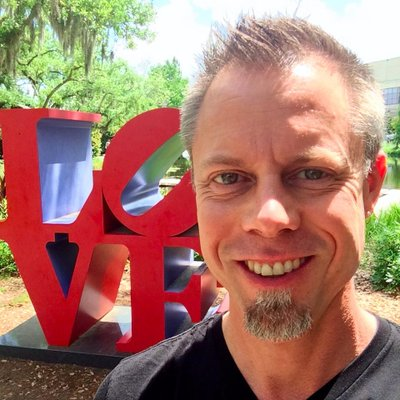
\includegraphics[width=10em]{rkasper.png}
  \end{center}
  \vspace{-2em}
\end{wrapfigure}

Richard Kasperowski défend l'idée que tous les développeurs et que toutes les équipes sont excellentes. Il intervient
en tant que Coach en transformation des entreprises, Coach agile et facilitateur en Open Space en aidant les gens, 
les équipes et les organisations à comprendre ce qu'ils ont a disposition, à identifier et à aligner ce qu'ils souhaitent
et à transformer ce qu'ils ont en ce qu'ils veulent. En tant que coach, manager et coéquipier, il a travaillé avec les 
plus grandes (et les plus petites) entreprises technologiques du monde en les aidait à améliorer leurs résultats.

Suivez Richard sur Twitter sur @rkasper, apprenez-en plus sur lui sur \url{https://kasperowski.com/}
et écrivez-lui sur richard@kasperowski.com.

\end{document}
